\section{System Design}\label{sec:sys_design}

\begin{figure}
    \centering
    \subfloat[][Quartus Prime RTL view\label{fig:fpga_rtl}]{
        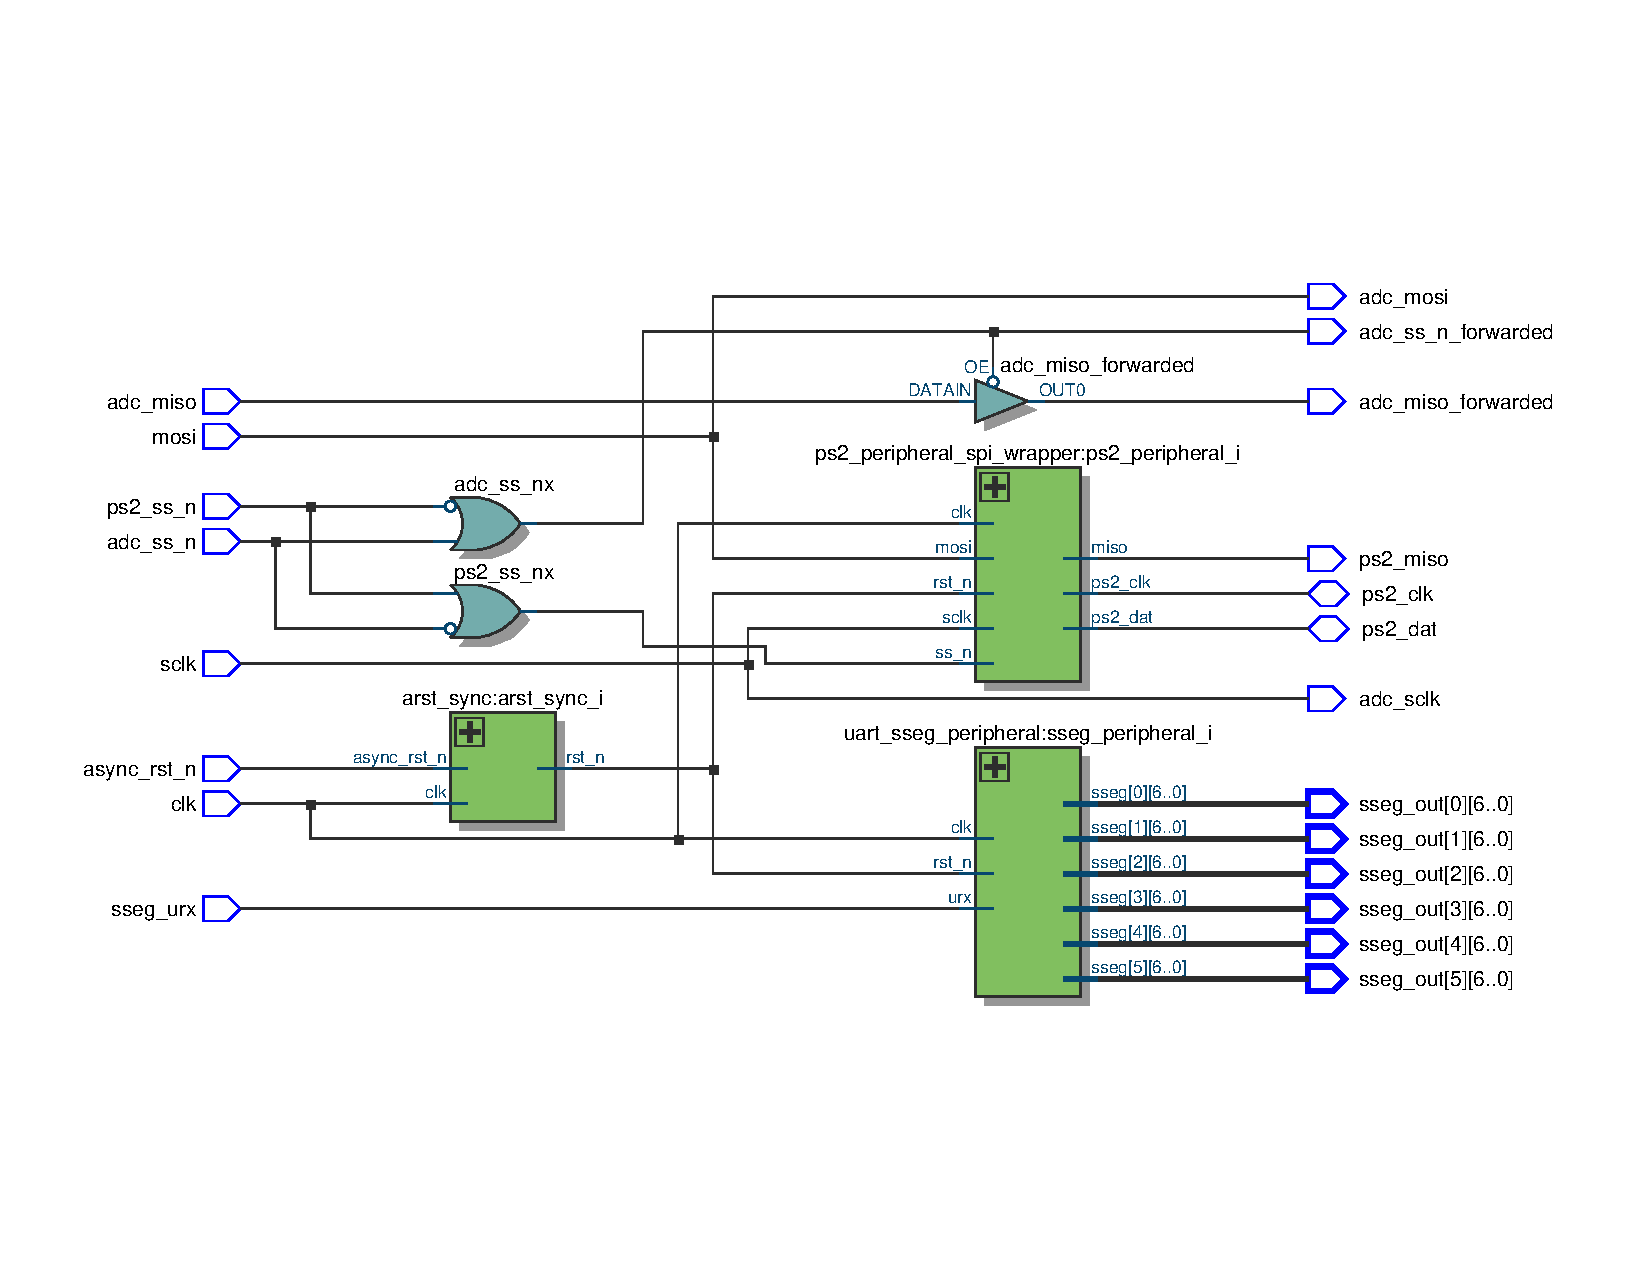
\includegraphics[width=\linewidth]{../gfx/RTLview.pdf}
    }\\
    \subfloat[][Signals mapped to the 2x20 header for interfacing with the MCU\label{fig:fpga_port}]{
        \includegraphics[scale=.65]{../gfx/GPIOHeader.eps}
    }
    \caption{DE1-SoC board subsystems}
    \label{fig:de1_soc}
\end{figure}

\begin{figure}
    \centering
    \includegraphics[width=.65\linewidth]{../gfx/mcu_pinout.png}
    \caption{Microcontroller pinout (generated by STM32CubeMX~\cite{cubemx}).}
    \label{fig:mcu_pins}
\end{figure}

\begin{figure}
    \centering
    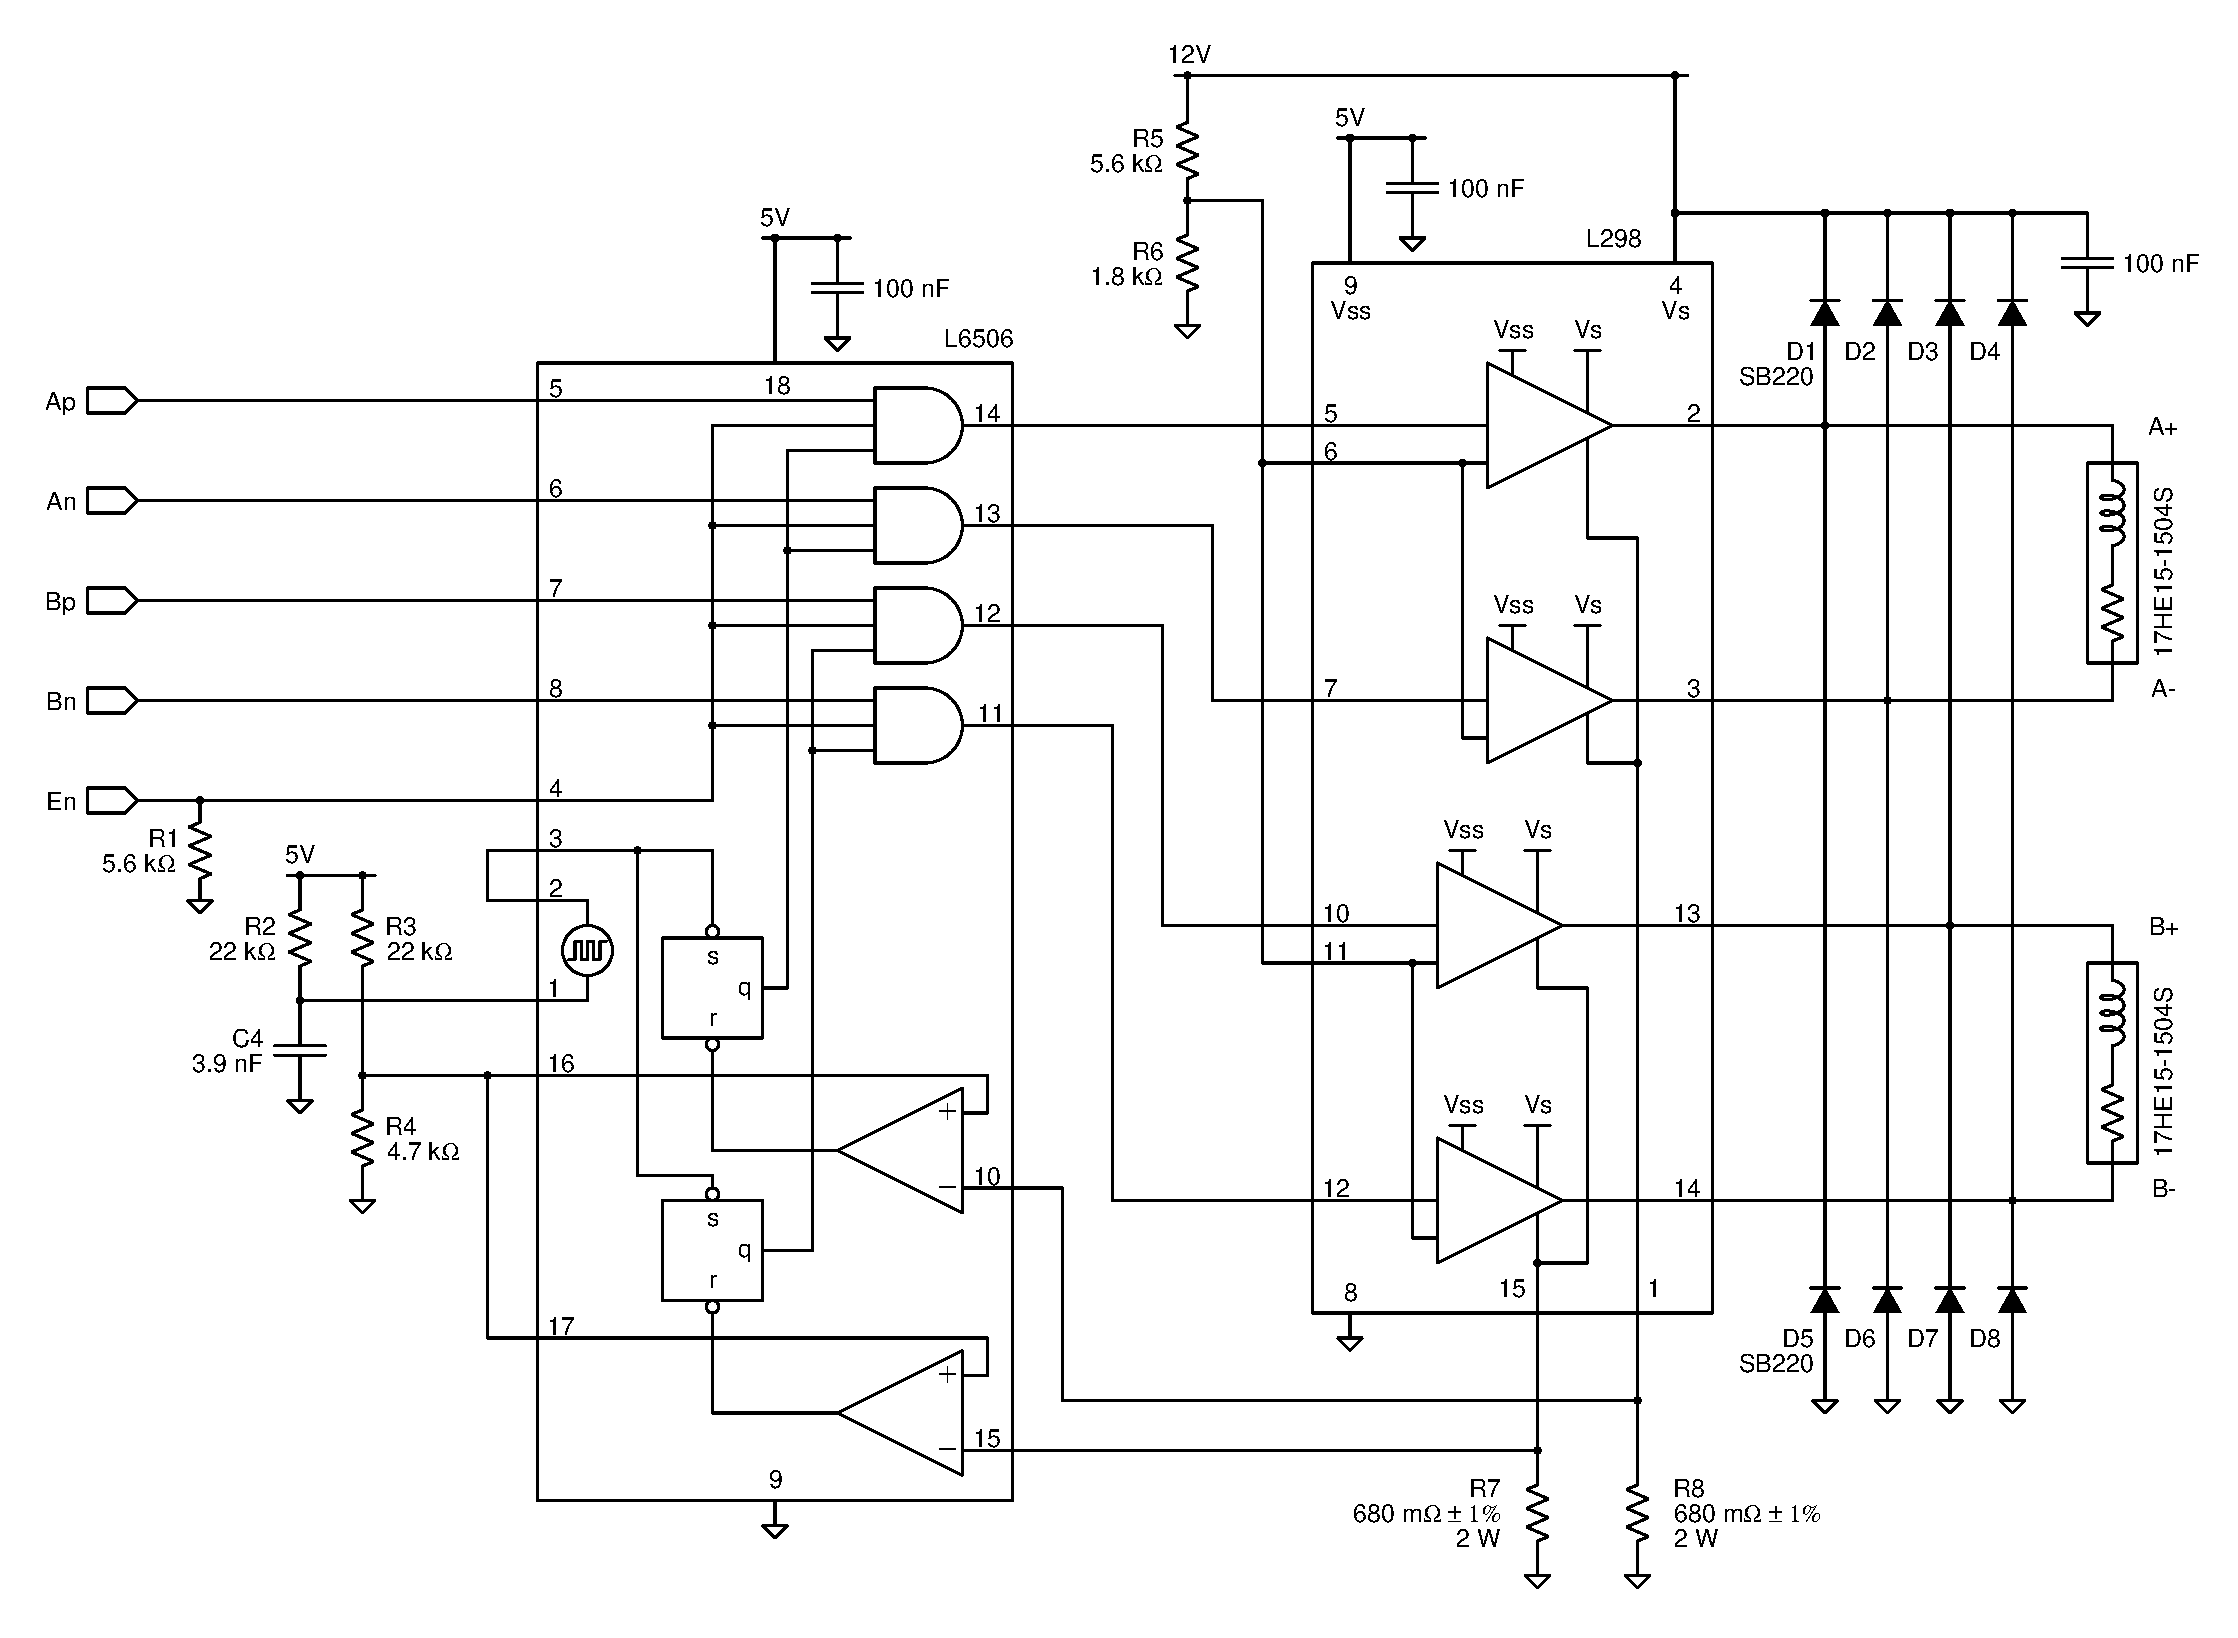
\includegraphics[width=.8\linewidth]{../gfx/motor_board.eps}
    \caption{Drive circuit for the bipolar stepper motor. The L6506 senses and controls the current in the motor windings, which are energized with the dual full-bridge driver L298.}
    \label{fig:motor_bd}
\end{figure}

The system is devised to target the hardware available on the design platform employed for the laboratory activities of the course, the DE1-SoC development kit by Terasic~\cite{de1soc}. The platform is built around Altera's Cyclone V SE SoC device~\cite{cyclone}, which integrates an ARM-based \ac{hps} tied to the FPGA fabric with an on-chip interconnect.
Potentially, this kit alone allows to experiment with digital processing in the form of software running on a hard or soft microprocessor to program hard and soft peripherals, as well as by synthesizing dedicated hardware. Despite this flexibility, the processor system is implemented with an external microcontroller development board, the NUCLEO-F401RE by STMicroelectronics~\cite{nucleo}, thus creating the opportunity to investigate communication protocols for wired interconnections.
As illustrated in the block diagram of~\cref{fig:sys}, the system comprises:
\begin{itemize}
    \item Input devices.
    \begin{itemize}
        \item The user and reset push buttons are part of the microcontroller development board.
        \item The linear potentiometer is wired to the ADC available on the DE1-SoC board, through the dedicated 2x5 header. This is discussed in~\cref{subsec:adc}.
        \item The PS/2 keyboard is attached to the corresponding port on the DE1-SoC board, through the fitted 6-pin mini-DIN connector.
    \end{itemize}
    
    \item Peripherals and glue logic implemented on the FPGA target, as more accurately shown in~\cref{fig:fpga_rtl}.
    The interface to the microcontroller consists of the signals mapped to the 2x20 expansion header GPIO0, as depicted in~\cref{fig:fpga_port}.
    \begin{itemize}
        \item The SPI-compatible port of the converter is routed through the FPGA fabric, up to the GPIO0 header.
        \item An asynchronous reset signal driven by the microcontroller is brought into the FPGA \qty{50}{\MHz} clock domain, to be used as a synchronously deasserted system-wide reset.
        \item The PS/2 peripheral implements the PS/2 protocol to communicate with the keyboard device, while it exposes an SPI port to the microcontroller. The design of the module is presented in~\cref{subsec:ps2}.
        \item The display peripheral drives the 7-segment displays available on the DE1-SoC board with the character stream received from the microcontroller via UART. This is discussed in~\cref{subsec:sseg}.
    \end{itemize}
    The slave select inputs are internally pulled up, to ensure an inactive level while the microcontroller resets.

    The blocks are modeled in SystemVerilog and are functionally simulated with testbenches that make use of the verification subset of the language. The approach to verification is directed testing, with non-constrained randomized stimuli. As a result, the testbenches can be run with the freeware edition of Questa Intel Starter FPGA Edition.
    The synthesis flow is carried out with the Quartus Prime Lite toolchain, using bash and Tcl automation scripts.

    \item Microcontroller and bipolar stepper motor drive circuit, as illustrated in greater details in~\cref{fig:mcu_pins,fig:motor_bd}.
    The microcontroller development board, the L6506 controller~\cite{l6506}, and the logic section of the L298 driver~\cite{l298}, are powered at \qty{5}{\V} from the DE1-SoC board; the microcontroller power supply is further regulated down to \qty{3.3}{\V}.
    \begin{itemize}
        \item As the FPGA I/Os are configured in the \qty{3.3}{\V} LVTTL standard, the microcontroller directly interfaces to the signals on the 2x20 header GPIO0. Notably, the PS/2 and ADC MISO signals are wired as a shared line into the microcontroller, and the input is internally pulled down to ensure a well-defined logic level while neither slave is selected.

        Several peripherals are configured to achieve the desired functionality, most importantly:
        \begin{itemize}
            \item The GPIO, to detect push button presses, as well as for generating reset and enable signals for the FPGA subsystem and its peripherals.
            \item The SPI3, USART1, and DMA2 to communicate with the peripherals synthesized in the FPGA.
            \item The TIM1 and DMA2, to generate two pairs of complementary square waveforms, with one pair in quadrature to the other, to drive the bipolar stepper motor.
        \end{itemize}
        Furthermore, one sector of the embedded NOR flash memory is used as a non-volatile circular buffer to store the motor movement pattern, and play it on demand. The architecture of the firmware is further explained in~\cref{sec:sw_design}.
        
        \item The L6506 inputs accept \qty{5}{\V} TTL levels, with $V_\text{IL} = \qty{0.8}{\V}$ and $V_\text{IH} = \qty{2}{\V}$. Consequently, the microcontroller can reliably drive them, without requiring any additional translation logic. During reset, the enable signal is pulled down with an external resistor and forces a motor brake.

        \item The L298 is permanently enabled. The datasheet prescribes that the enable signals of the H-bridges are to be driven low before turning on or off the power stage, which is achieved by means of the resistive divider $(R_5,\,R_6)$. 
    \end{itemize}
    The design of the circuit, for the bipolar stepper motor 17HE15-1504S~\cite{stepp}, is discussed in~\cref{subsec:motor_bd}.
\end{itemize}

\subsection{Angular Velocity Acquisition}\label{subsec:adc}

Depending on the board revision, the ADC is either the AD7928~\cite{ad7928} or the LTC2308~\cite{ltc2308}, which feature \qty{12}{\bit} of resolution with a successive approximation topology, and an SPI-compatible serial interface. The analog input range changes slightly between the two devices: for the AD7928, the full range can be digitally selected equal to the external \qty{2.5}{\volt} nominal reference or double its value. For the LTC2308 instead, it is fixed to \qty{4.096}{\volt}. In either case, the 2x5 dedicated header only provides access to the eight input channels, to the ground, and to the \qty{5}{\volt} supply rail, thus preventing measurements in a ratiometric configuration.
    
Accordingly, for the AD7928, a \qty{10}{\kohm} linear potentiometer is wired between the \qty{5}{\volt} supply rail and ground, with the wiper node connected to a single-ended input channel. The \qty{500}{\uA} nominal current through the voltage divider makes the \qty{1}{\uA} leakage current negligible.
In the worst case scenario for the sample and hold circuitry, the wiper of the potentiometer sits at halfway position, such that the output resistance of the thevenin equivalent $R_\text{s}$ is at its maximum value of \qty{2.5}{\kohm}. 
In this condition, with a typical hold capacitance $C_\text{h}$ of \qty{20}{\pF} and an equivalent input resistance $R_\text{in}$ of \qty{400}{\ohm}, a fully discharged hold capacitor charges up to the \qty{2.5}{\volt} input $V_\text{s}$ following
\[
    v_\text{h}\pqty*{t} = V_\text{s}\,\pqty*{1-e^{-t/\tau}}
    ,\qquad \text{with}\qquad \tau = \pqty*{R_\text{s}+R_\text{in}}\,C_\text{h}
\]
and the time required for this voltage to settle within half LSB of the final value is
\begin{equation}\label{eq:tset}
    t_\text{set} = \tau\,\ln\,\frac{V_\text{s}}{0.5 \,\text{LSB}}
\end{equation}
Hence, $t_\text{set} = \qty{482}{\ns}$ bounds the minimum acquisition time for achieving full resolution conversions.

Considering the narrower analog range of the LTC2308, the \qty{10}{\kohm} potentiometer is wired at the bottom of a voltage divider, with the resistor $R_1$ on the upper branch sized to limit the voltage drop on the potentiometer. Denoting with $V_\text{s}$ the supply voltage and with $V_\text{fr}$ the ADC full range, it must hold
\[
    V_\text{s}\,\frac{R_\text{pot}}{R_\text{pot} + R_1} \le V_\text{fr}
\]
Therefore, in the typical case for the supply and full range voltages, but considering a \qty{10}{\percent} uncertainty on the potentiometer resistance and a \qty{1}{\percent} uncertainty for $R_1$, it is required that
\[
    R_{1,\text{min}} \ge 
    R_{\text{pot},\text{max}}\,\pqty*{\frac{V_\text{s}}{V_\text{fr}}-1}
\]
which yields $R_1 \ge \qty{2.43}{\kohm}$. Accordingly, $R_1$ can be chosen in the E12 series with a nominal value of \qty{2.7}{\kohm}.
Finally, the observation on the minimum acquisition time for the AD7928 applies here too. Given the different configuration of the voltage divider, the output resistance is maximized when the wiper reaches a position where the total divider resistance is split in half, hence $R_\text{s}$ is \qty{3.18}{\kohm}. Considering the equivalent model of the analog input, with a typical hold capacitance $C_\text{h}$ of \qty{55}{\pF} and an equivalent input resistance $R_\text{in}$ of \qty{100}{\ohm}, \cref{eq:tset} yields $t_\text{set} = \qty{1.53}{\us}$.

The four signals of the ADC serial interface are routed through the FPGA fabric up to the 2x20 GPIO0 expansion header, where they connect to the microcontroller pins assigned to the SPI peripheral. The peripheral is configured as a full-duplex master, with software-controlled slave select signals.

\subsection{Angular Displacement Acquisition}\label{subsec:ps2}

\begin{figure}
    \centering
    \subfloat[][System receiving data. The device generates data while the clock is high.]{
        \includegraphics[width=.7\linewidth]{../gfx/ps2_timing_rx.eps}
    }\\
    \subfloat[][System sending data. The system generates data while the clock is low; following the parity bit, the device detects the stop bit and pulls the data line low while the clock is high (dashed portion of the waveform).]{
        \includegraphics[width=.9\linewidth]{../gfx/ps2_timing_tx.eps}
    }
    \caption{PS/2 timing diagrams. The clock period ranges from \qtyrange{60}{100}{\micro\s}; the maximum request-to-send duration is \qty{15}{\milli\s}.}
    \label{fig:ps2_timing}
\end{figure}

The PS/2 protocol~\cite{ps2_controller,ps2_device} regulates the point-to-point bidirectional communication between the system and the keyboard device. It is a synchronous serial protocol in which data is time-multiplexed over a single data line, while a dedicated line carries the clock signal. Accordingly, the communication is half-duplex and both clock and data lines are shared with an open-drain architecture to avoid damage in case of conflicts.

The clock is always generated by the PS/2 device, but the system can pull the clock line low to inhibit the bus, potentially causing collisions that are used to abort ongoing transmissions in either direction. When the bus is not inhibited, two configurations are possible prior to a transmission: if the data line is also pulled high, the bus is in its idle state, which is the only one in which the device can initiate a transmission to the system. Alternatively, if the data line is held low by the system, the configuration signals the device that the system is ready to transmit data and awaiting clock generation.
The transmission is character-based and the frame comprises:
\begin{itemize}
    \item Start bit, always 0
    \item \qty{8}{\bit} character, transmitted LSB first
    \item Odd parity bit, either 0 or 1 such that the overall count of bits with value 1 in the character concatenated with the parity bit is odd
    \item Stop bit, always 1
\end{itemize}
The timing diagram for receiving and sending data are shown in~\cref{fig:ps2_timing}.

\subsubsection{PS/2 Peripheral}

\begin{figure}
    \centering
    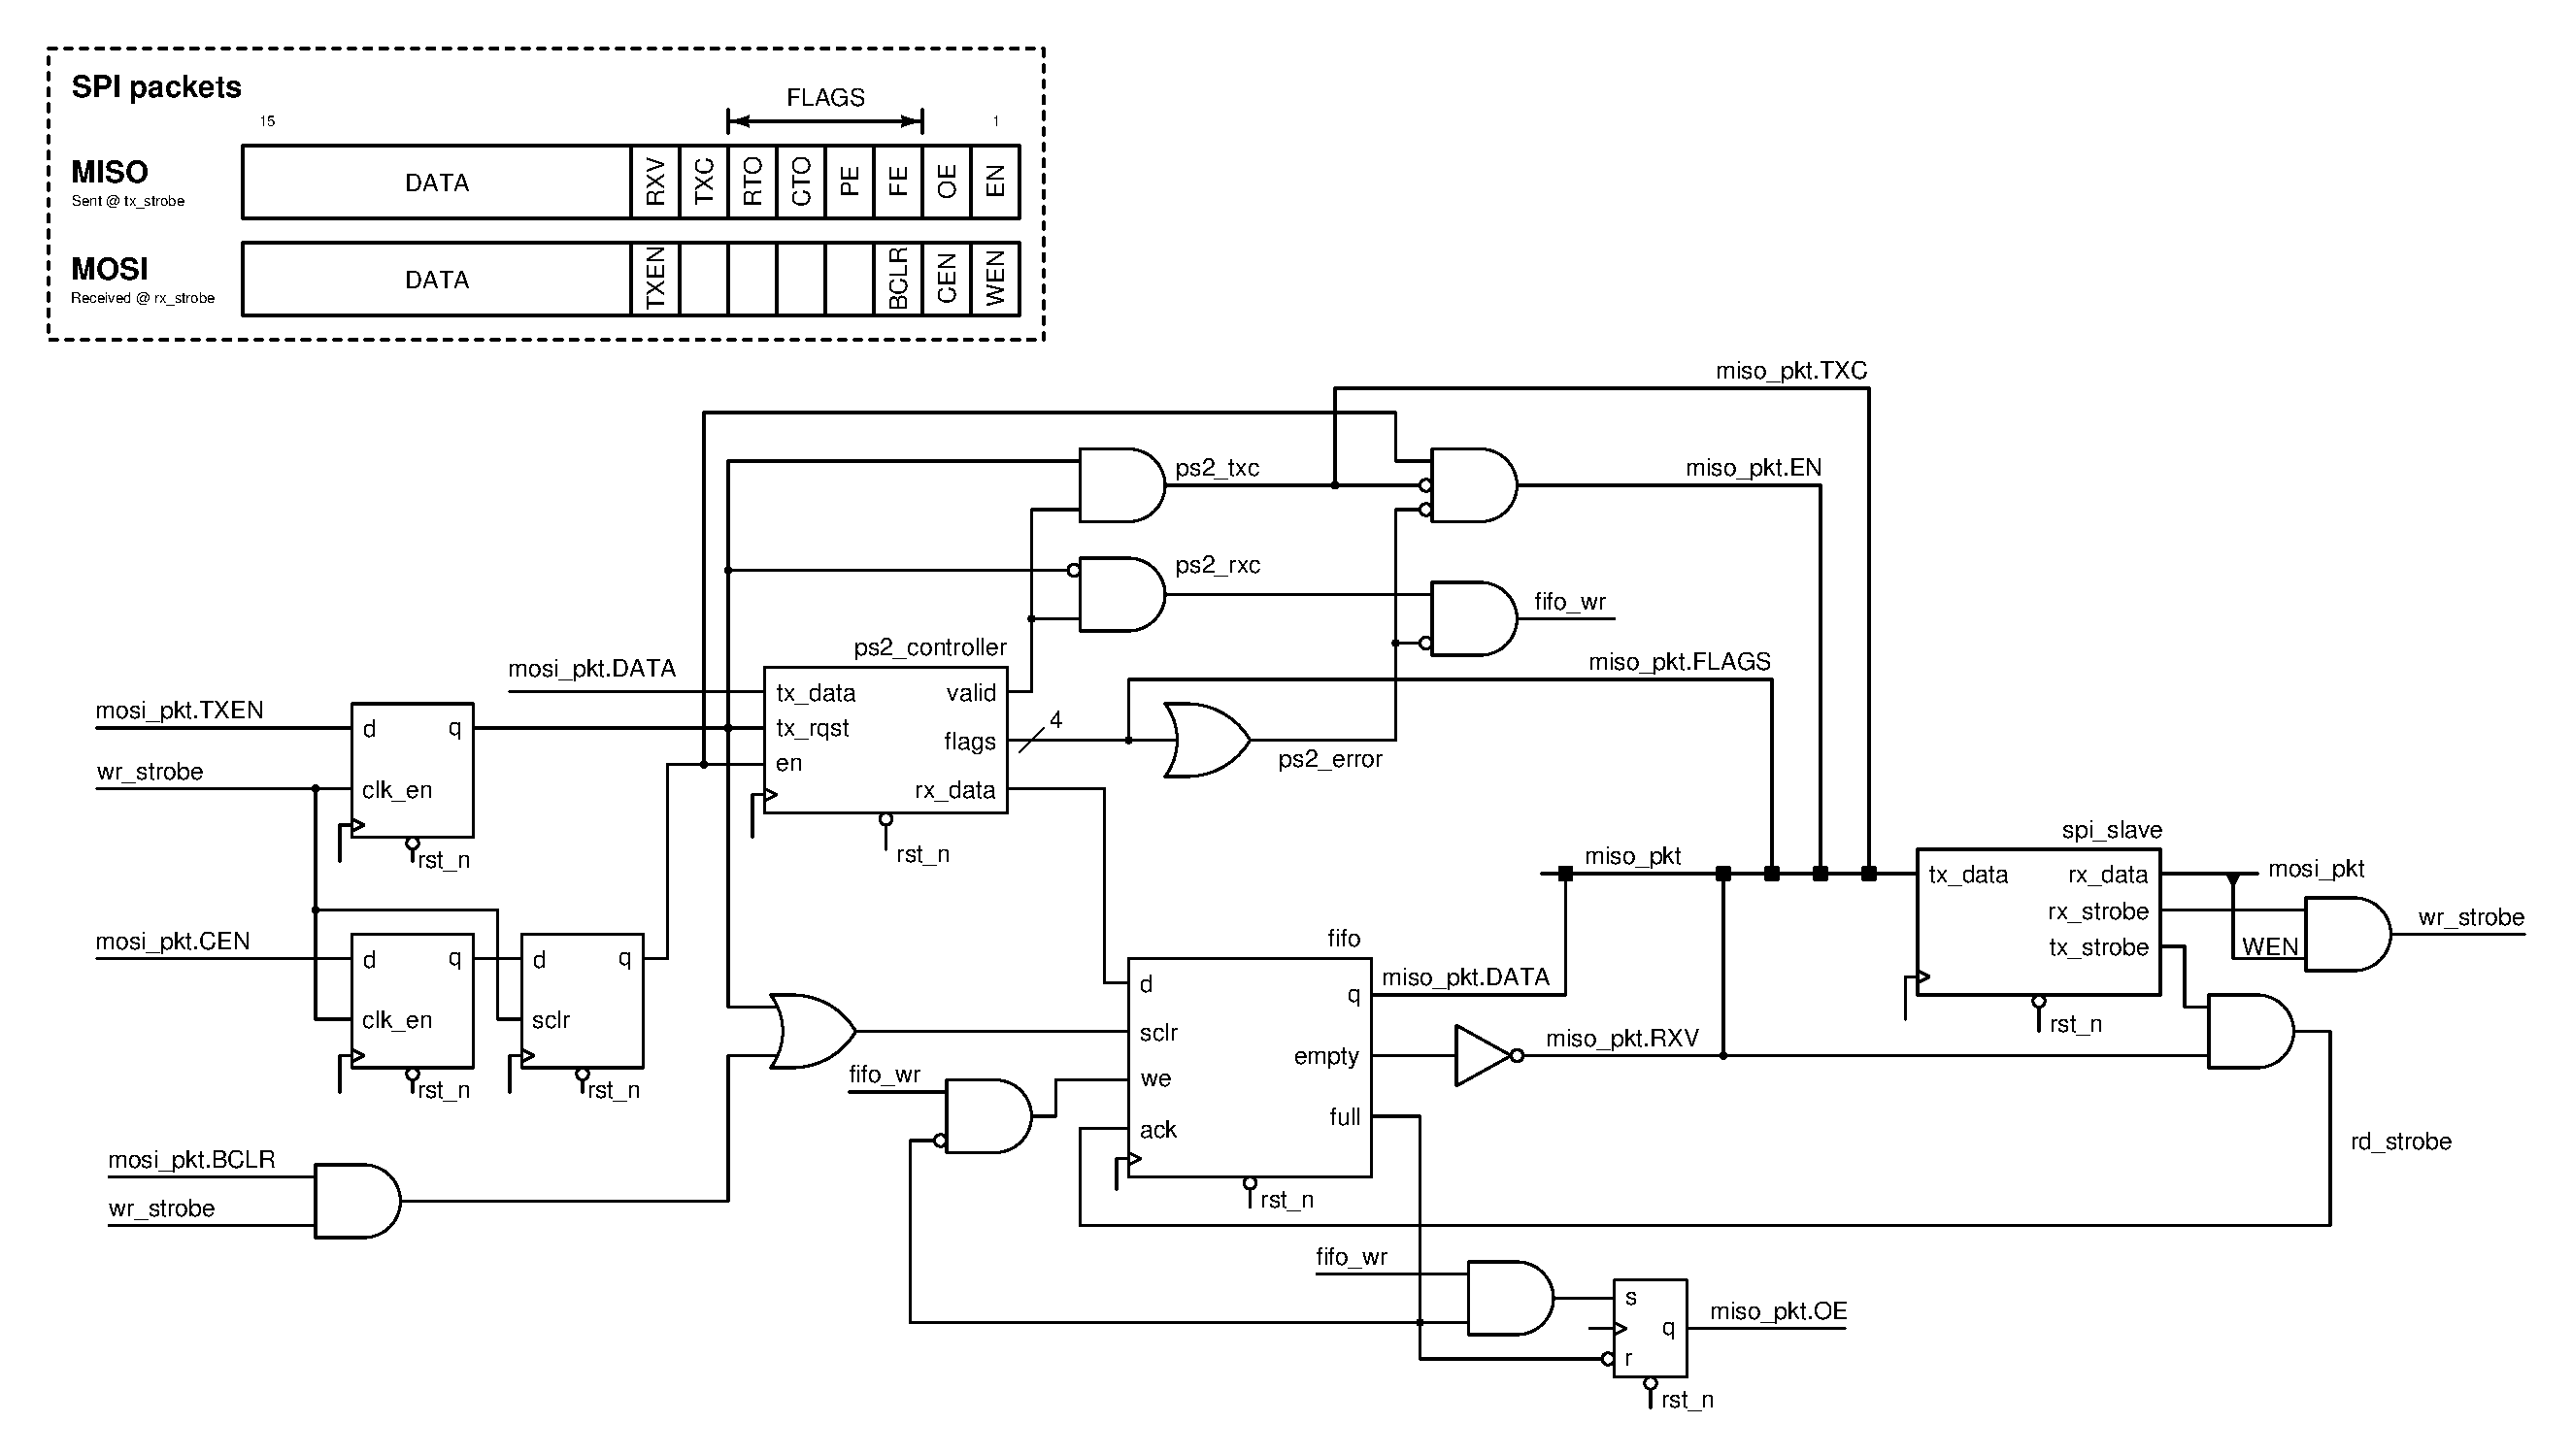
\includegraphics[width=\linewidth]{../gfx/ps2_peripheral_spi_wrapper.eps}
    \caption{SPI-compatible PS/2 controller peripheral design. The module implements the PS/2 protocol for exchanging data with a PS/2 device, exposing its control, status, and data registers through SPI. Data received from the device is buffered in an SRAM FIFO. The PS/2 and SPI buses are not shown.}
    \label{fig:ps2_peripheral}
\end{figure}

The PS/2 protocol is implemented by the custom peripheral shown in~\cref{fig:ps2_peripheral}, which enables data exchange with an external PS/2 device, under the control of an SPI-capable system. It includes three key modules: a PS/2 controller, a show-ahead single-clock FIFO, and an SPI slave controller. Additional glue logic implements the desired behavior for the control and status register bits that are exposed through SPI.

\begin{description}
    \item[PS/2 Controller] It implements the PS/2 protocol specifications and provides an higher-level simplified interface to the PS/2 device, as presented in~\cref{lst:ps2_controller}. It supports bidirectional communication and provides several reliability features. The data and clock lines are synchronized to the system clock domain with a flip-flop chain: the depth defaults to 2, which achieves a reasonable trade-off of latency and \ac{mtbf} due to metastable events. The controller detects:
    \begin{itemize}
        \item Frame errors. On reception, if the start or stop bit is missing at the expected time. On transmission, if the acknowledgment bit is similarly absent.
        \item Parity error, if the parity check fails during reception.
        \item Clock timeouts, if the falling edges of the clock are separated by more than \qty{150}{\micro\s} during either reception or transmission.
        \item Request timeouts. On transmission, if the device does not generate the clock within a \qty{15}{\milli\s} window after the system inhibits the PS/2 bus (see~\cref{fig:ps2_timing}).
    \end{itemize}
    
    The controller has been designed according to the ASM methodology, starting from a pseudocode description of the receive and transmit operations; the resulting ASM chart and data path are provided in~\cref{apx:ps2_controller}. In summary, the module operates as follows.
    \begin{itemize}
        \item On reset or while not enabled, the controller inhibits the bus by driving the clock line low.
        \item While enabled, with no pending transmission request, the controller monitors the bus for transmissions from the device. In case of successful reception, the valid signal pulses for one clock cycle and the received character appears on the data output. Conversely, in case of failure, the valid signal is held high while the flags signal the cause. While in this failure state, the PS/2 bus is inhibited; resuming normal operation requires a falling transition on the enable signal.
        \item While enabled, with no ongoing transmission to the device, the controller samples the data to be transmitted in the same clock cycle where the transmission request gets asserted. In case of successful transmission, the valid signal is held high until the request signal becomes inactive, and the bus is inhibited. Conversely, the failure behavior is the same as in reception.
    \end{itemize}

    \begin{listing}
    \begin{minted}{systemverilog}
    module ps2_controller #(
      parameter int unsigned SYNC_STAGES = 2,
      parameter real FCLK_HZ = 50e6,
      parameter int unsigned TIM_PSC = 249 // tim_fclk = fclk/(PSC+1) = 200 kHz, for 50 MHz clock
    ) (
      input var logic clk,
      input var logic rst_n,
      input var logic en,
    
      input var logic tx_rqst,
      input var logic [7:0] tx_data,
    
      output logic valid,
      output logic [7:0] rx_data,
      output ps2_pkg::flags_t flags,
    
      inout tri ps2_clk,
      inout tri ps2_dat
    );
    \end{minted}
    \caption{SystemVerilog interface of the PS/2 controller. The number of flip-flop synchronizing stages for the PS/2 lines is parameterized and defaults to 2. The timing thresholds are computed at compile-time, based on the specified clock frequency and prescaler value.}
    \label{lst:ps2_controller}
    \end{listing}

    \item[Show-Ahead Single-Clock FIFO] Data received from the PS/2 device is buffered in a synchronous FIFO structure with a show-ahead interface. Provided that the empty signal is inactive, this interface automatically outputs the first valid word, and asserting the read-acknowledge signal causes the FIFO to output the next valid word.

    The module is designed to infer embedded dual-port SRAM blocks if available, without depending on a specific read-during-write behavior. On reset, the read and write pointers are cleared, and the FIFO is empty. With the first write operation, the data is stored at the write pointer location, which is the same one being read: due to the read-during-write event, the SRAM may output the old data, thus the latency for the data to appear at the output is 2 clock cycles. Accordingly, the empty flag is cleared with the same latency. The full design is provided in~\cref{apx:fifo}.

    \item[SPI Slave Controller] It implements the SPI protocol in the slave role, with programmable frame length, clock polarity (CPOL) and clock phase (CPHA).

    To decrease clock oversampling requirements, the receive and transmit logic operate within the domain of the external SPI clock, generated by the master device; the slave select signal crosses into the system clock domain with a dual flip-flop synchronizer. While the slave is not selected, the data to be transmitted is sampled in the system clock domain up to one clock cycle before the transmit strobe signal pulses high, which marks the start of communication. At the end of the communication, when the slave is deselected, the received data is loaded onto the data output and becomes valid in the system clock cycle when the receive strobe signal pulses high.
    \Cref{apx:spi} contains the design of the module and the manual timing analyses.
    
\end{description}

The peripheral exposes its control, status, and data registers as packets exchanged through SPI, according to the format summarized in~\cref{fig:ps2_peripheral}. A detailed description of the packets format is provided below.
\begin{description}[style=nextline]
    \item[MOSI Packet]\hfill
    
        \begin{enumerate}[
            label=\emph{Bit \arabic*}, widest=s 15:8,
            left=\parindent, align=left,
            itemsep=2.5\itemsep,
            start=0
        ]
        \item \textbf{WEN}: Write Enable
        \begin{enumerate}[label=\arabic*:, start=0]
            \item The packet is discarded
            \item The packet is decoded
        \end{enumerate}
    
        \item \textbf{CEN}: Controller Enable
        \begin{enumerate}[label=\arabic*:, start=0]
            \item Disables the controller and inhibits the PS/2 bus (clock line low)
            \item Clears the flags (FE, PE, CTO, and RTO), and enables the controller in the operation mode set by TXEN.
            
            If the controller is already running (EN bit is set), the current operation is aborted. Aborting a receive operation while the PS/2 device is transmitting a character generates a communication error (FE, PE, or CTO set).
        \end{enumerate}
    
        \item \textbf{BCLR}: Buffer Clear
        \begin{enumerate}[label=\arabic*:, start=0]
            \item The receive FIFO buffer is not flushed
            \item The receive FIFO buffer is flushed. If both CEN and BCLR are set, the flush operation is performed prior to enabling the controller.
        \end{enumerate}
    
        \makeatletter
            \addtocounter{\@enumctr}{4}
        \makeatother
        
        \item \textbf{TXEN}: Transmitter Mode Enable
        
        This bit determines the operation mode.
        \begin{enumerate}[label=\arabic*:, start=0]
            \item The controller receives data from the PS/2 device.
            Incoming packets are stored in the FIFO buffer, whose state is represented by the RXV and OE status bits. When the FIFO is empty, the RXV bit is cleared and the DATA field is undefined. Otherwise, the RXV bit is set, and the DATA field is valid. If the FIFO buffer is full and new packets are received, the OE status bit is set. Each SPI transfer removes one element from the FIFO, which may also clear the OE bit. Alternatively, the OE bit is cleared by flushing the FIFO buffer when the BCLR control bit is set.
    
            \item The FIFO buffer is cleared, and the controller sends data to the PS/2 device. When the operation completes, the TXC bit is set, the flags are updated (FE, CTO, and RTO), the EN bit is cleared and the PS/2 bus is inhibited (clock line low).
        \end{enumerate}
    
        \item[\emph{Bits 15:8}] \textbf{DATA}: Transmit Data
        
        If TXEN is set, the data to be sent to the PS/2 device.
    \end{enumerate}
    
    \item[MISO Packet]\hfill
    
        \begin{enumerate}[
            label=\emph{Bit \arabic*}, widest=s 15:8,
            left=\parindent, align=left,
            itemsep=2.5\itemsep,
            start=0
        ]
            \item \textbf{EN}: Controller Enabled
            
            This bit is set by the master when enabling the controller and is cleared by the hardware in one of the following cases:
            \begin{itemize}
                \item The communication has failed and a flag is set (FE, PE, CTO, or RTO).
                \item The TXEN control bit enabled the controller in transmitter mode, and the transmission has terminated (TXC is set).
            \end{itemize}
            With the EN bit cleared, the PS/2 bus is inhibited (clock line low).
            
            \item \textbf{OE}: Overrun Error
            
            This bit is set by the hardware when the FIFO buffer is full and a new packet has been received and lost. It is automatically cleared when removing elements from the FIFO with SPI transfers, when flushing the buffer by setting the BCLR bit, or when the controller is enabled in transmitter mode.
            
            \item \textbf{FE}: Frame Error
    
            This bit is set by the hardware if the communication has failed in one of the following ways. While receiving data from the PS/2 device, either the START or STOP bits are not recognized at the expected time. While transmitting data, the ACK bit is not recognized at the expected time.
            
            Once the error is raised, the controller halts and inhibits the PS/2 bus (clock line low). Resuming normal operation requires enabling the controller again.
            
            \item \textbf{PE}: Parity Error
            
            This bit is set by the hardware if the parity check on the data received from the PS/2 device has failed.
            
            Once the error is raised, the controller halts and inhibits the PS/2 bus (clock line low). Resuming normal operation requires enabling the controller again.
            
            \item \textbf{CTO}: Clock Timeout
    
            This bit is by the hardware if the falling edges of the clock generated by the PS/2 device are separated by more than \qty{150}{\micro\s}, during either reception or transmission.
            
            Once the error is raised, the controller halts and inhibits the PS/2 bus (clock line low). Resuming normal operation requires enabling the controller again.
            
            \item \textbf{RTO}: Request Timeout
    
            This bit is set by the hardware if, on transmission, the PS/2 device has failed to generate the clock within a \qty{15}{\milli\s} window after the PS/2 bus was inhibited.
    
            Once the error is raised, the controller halts and inhibits the PS/2 bus (clock line low). Resuming normal operation requires enabling the controller again.
            
            \item \textbf{TXC}: Transmission Complete
            This bit is set by the hardware when the controller was enabled in transmitter mode and the transmission has completed (with or without errors).
            
            \item \textbf{RXV}: Receive Data Valid
            This bit is set by the hardware when the DATA field is valid and contains one character received from the PS/2 device. The read operation from the FIFO is automatically acknowledged.
            
            \item[\emph{Bits 15:8}] \textbf{DATA}:
            
            If RXV is set, one character received from the PS/2 device.
            
        \end{enumerate}
\end{description}

\subsection{7-Segment Displays Peripheral}\label{subsec:sseg}

\begin{figure}
    \centering
    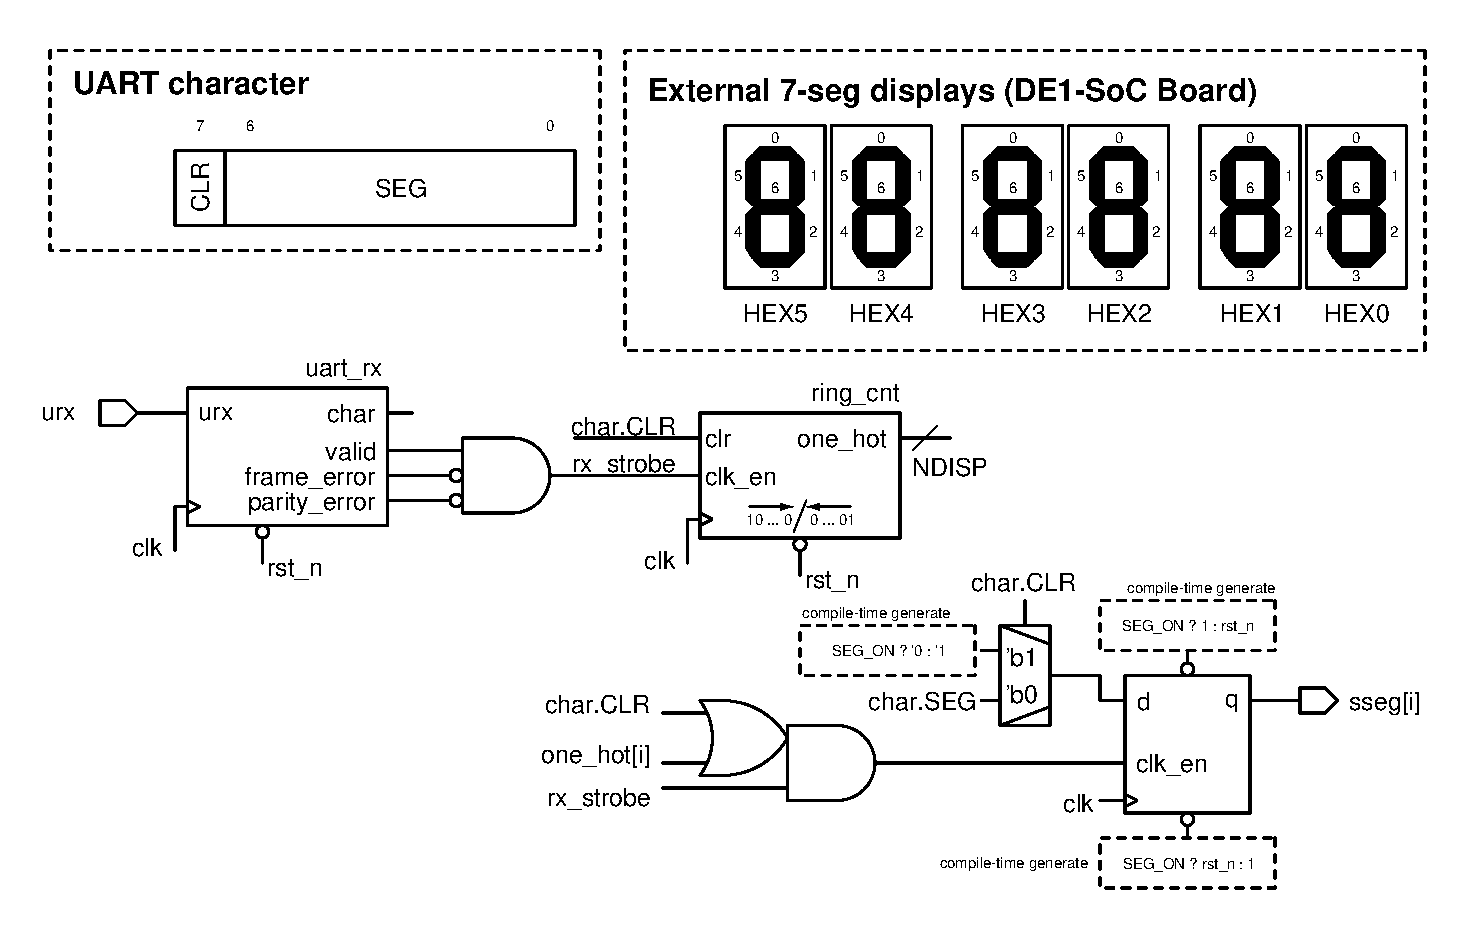
\includegraphics[width=.8\linewidth]{../gfx/display_peripheral.eps}
    \caption{Display peripheral design. The module circularly displays an UART character stream on a set of 7-segment displays.}
    \label{fig:disp_peripheral}
\end{figure}

The display peripheral is devised to serially control a set of 7-segment displays. It processes a stream of UART characters, where each character can either instruct the peripheral to clear all displays or update the input for a single display; one character after the other, the displays can be all updated in a rotating manner.
The design, shown in~\cref{fig:disp_peripheral}, makes use of a custom UART receiver module. When a transmission completes without frame or parity errors, the character appears on the output while the valid signal pulses high: the most significant bit of the character is decoded as the clear command. If the bit is set, the registers driving the display segments are forced into the off-state specified at compile-time, and the one-hot counter is cleared. Otherwise, the one-hot counter state is used to mask all clock-enable signals of the registers driving the display segments, except for one. This register is loaded with the received character data, while the one-hot counter shifts to point to the next display in the set.

\subsubsection{UAR(T) Core}

\begin{listing}
\inputminted{c}{../code/uart_RX.asm}
\caption{Pseudocode of the asynchronous receive operation for the ASM design metodology}
\label{lst:uart}
\end{listing}

The core implements a flexible asynchronous serial receiver for the NRZ-L encoding. It supports several compile-time programmable parameters:
\begin{itemize}
    \item Frame format:
    \begin{itemize}
        \item Character length
        \item Presence and type of parity (even or odd)
        \item Number of STOP bits
    \end{itemize}
    \item Baud rate, by specifying system clock, prescaler, and target clock frequency
    \item Serial line synchronizer depth, which determines the trade-off between data latency and \ac{mtbf} due to metastable events
\end{itemize}
In addition, it features clock synchronization on all transitions, besides the UART-mandated synchronization on the START bit.
Upon reception, the valid signal pulses high for one clock cycle, while the received character and error flags are latched on the outputs.

The module has been designed according to the ASM methodology, starting from the pseudocode in~\cref{lst:uart}; the resulting ASM chart and data path are provided in~\cref{apx:uart}.
 
\subsection{Bipolar Stepper Motor Drive Circuit}\label{subsec:motor_bd}

For educational purposes, the drive circuit does not employ fully integrated bipolar motor drivers. Instead, the L298 integrates two full-bridges to energize and reverse the phase currents. Additionally, the L6506 addresses the limitations of the simpler L/nR drive topology, in which the time constant of the inductive load is reduced by adding external resistances in series with the coils, while the desired asymptotic current is restored by increasing the drive voltage. To avoid the large power dissipation of the external resistances, the approach involves increasing the slew rate of the phase currents with an higher drive voltage, and limiting the phase currents by switching the driver. As shown in~\cref{fig:motor_bd}, the phase current is sensed on the return path from the H-bridge. During the low time of the oscillator period, the drive signals pass through. However, if the phase current exceeds the limit set by the reference voltage, the drive signals are gated for the remaining part of the period. The energy stored in the inductor is dissipated as the current recirculates in the lower half of the bridge: through one snubber diode, the coil resistance, the transistor in the opposite branch, and the sense resistance. Notice that, being possible to independently set the peak phase currents, this chopping circuit supports a microstepping drive technique.

The power output stage of the L298 operates from a fixed \qty{12}{\V} switching power supply~\cite{pwr}. By means of the $(R_5,\,R_6)$ divider, the enable signal pulls low as the supply voltage is about to turn on or off~\cite[9]{l298}. Considering the input characteristics and accounting for a sensible noise margin, it must hold:
\begin{gather*}
    V_\text{IH}+N_\text{MH} \leq V_\text{s}\,\frac{R_6}{R_5+R_6} \leq V_\text{ss} \\
    \frac{V_\text{s}}{R_5+R_6} \gg I_\text{IH}
\end{gather*}
To ensure that the enable signal pulls low in the widest range of the voltage supply dynamic, and assuming a \qty{5}{\percent} tolerance on the resistances, the nominal values in the E12 series can be chosen as:
\begin{align*}
&R_5 = \qty{5.6}{\kohm} &R_6 = \qty{1.8}{\kohm}
\end{align*}

The bipolar stepper motor 17HE15-1504S is rated for a phase current of \qty{1.5}{\A}, and is characterized by a coil resistance of \qty{2.3(.23)}{\ohm} and a coil inductance of \qty{4(.8)}{\mH}. Working with a \qty{10}{\percent} derating factor, the current driven by the L298 is limited to \qty{1.35}{\A} per channel: in the worst case of a total saturation voltage $V_\text{CEsat} = \qty{4.9}{\V}$, the total power dissipated by the driver amounts to \qty{13.23}{\W}.
Now, for the multiwatt15 package in free air, the temperature at the junction would rise above the ambient temperature by:
\[
    \Delta T = R_{\theta\text{ja}}\;P_\text{tot} \approx \qty{463}{\celsius}
\]
hence, the need to lower the thermal resistance with an heat sink. Common heat sinks for this form factor are made of 6063-T5 aluminum alloy, which has a typical thermal conductivity $\kappa$ of \qty{209}{\W\per{\m\kelvin}} (for instance, \cite{xsd_hs}). From the mechanical data of the package, the minimum contact area $S$ to the heat sink is \qty{338.1}{\milli\meter\squared}; therefore, the thermal resistance across the contact area, for an average thickness $\Delta l$ of \qty{5.52}{\milli\m} is:
\[
    R_{\theta\text{sa}} = \frac{\Delta l}{\kappa S} \approx \qty{78.2e-3}{\celsius\per\W}
\]
Finally, by using a thermal compound to improve the thermal coupling between the case and the heat sink, it is reasonable to achieve:
\[
    R_{\theta\text{cs}} \approx \qty{0.5}{\celsius\per\W}
\]
In conclusion, the driver is expected to work at a maximum ambient temperature of:
\[
    T_{\text{a,max}} = T_{\text{j,max}} 
        - \pqty*{R_{\theta\text{jc}}+R_{\theta\text{cs}}+R_{\theta\text{sa}}}
        \;P_\text{tot} \approx \qty{83}{\celsius}
\]
which covers the broadly accepted range for consumer electronics from \qtyrange{0}{70}{\celsius}.

For the current recirculation paths, the datasheet advises selecting fast-switching snubber diodes, preferably of Schottky type. A family of suitable devices is the SB2x0~\cite{sb260}, which are rated for a maximum average forward current of \qty{2}{\A}. As a first approximation, the supply voltage of the power output stage, plus one forward voltage drop of the snubber diode during clamping, bounds the maximum reverse voltage. As a consequence, the SB220 can be selected for the circuit.

The sense resistors must be sized to comply with the maximum allowable voltage at the sensing pins, equal to \qty{2}{\V}. Considering a \qty{680(6.8)}{\mohm} resistor rated for \qty{2}{\W}~\cite{rsense}, the nominal voltage drop for the chosen maximum phase current of \qty{1.35}{\A} is \qty{918}{\mV}. In this condition, the resistor dissipates \qty{1.24}{\W}: computing the thermal resistance from the power derating curve in the datasheet:
\[
    R_\theta = \frac{\qty{155}{\celsius}-\qty{70}{\celsius}}{\qty{2}{\W}}
             = \qty{42.5}{\celsius\per\W}
\]
it is possible to evaluate the effect of self-heating. In the worst case of the \qtyrange{0}{70}{\celsius} temperature range, the resistor heats to:
\[
    T_\text{r,max} = T_{\text{a,max}} + R_\theta\;P \approx \qty{123}{\celsius}
\]
Consequently, from the temperature coefficient $\alpha = \qty{300}{\ppm\per\celsius}$:
\[
    \Delta R_\text{sh} = R_0\,\alpha\,\pqty*{T_\text{r,max} - T_\text{r}0}
    \approx \qty{19.9}{\mohm}
\]
which shows that the self-heating effect dominates the uncertainty. Accordingly:
\[
    R_7 = R_8 = \qty{680(27)}{\mohm}
\]

The sensed voltage is used in the L6506 to implement the constant current drive. In the worst case, the phase current reaches the maximum value of \qty{1.35}{\A} and the sensed voltage at the comparator input is \qty{882}{\mV}. As a consequence, the major constraints are:
\begin{gather*}
    V_\text{ss}\,\frac{R_4}{R_3+R_4} \leq \qty{882}{\mV} \\
    \frac{V_\text{ss}}{R_3+R_4} \gg I_\text{IB}
\end{gather*}
Having already derated the maximum phase current, the constraint can be evaluated for the nominal resistance values. An optimal selection is:
\begin{align*}
    &R_3 = \qty{22}{\kohm} &R_4 = \qty{4.7}{\kohm}
\end{align*}
In fact, with \qty{1}{\percent} uncertainties, the worst case voltage reference would be \qty{895}{\mV}, which corresponds to a maximum phase current of \qty{1.37}{\A}.
In addition, the phase current may exceptionally increase above the chosen peak value during the active time of the oscillator waveform, as the driving inputs cannot be masked. With the same selection of $(R_2,\,C_4)$ as in the application circuit~\cite[5]{l6506}, the nominal frequency of the oscillator is \qty{16.9}{\kHz} and the nominal active time lasts \qty{2.57}{\micro\s}.
